% !TEX TS-program = pdflatex
% !TEX encoding = UTF-8 Unicode

% This is a simple template for a LaTeX document using the "article" class.
% See "book", "report", "letter" for other types of document.

\documentclass[20pt]{article} % use larger type; default would be 10pt

\usepackage[utf8]{inputenc} % set input encoding (not needed with XeLaTeX)

%%% Examples of Article customizations
% These packages are optional, depending whether you want the features they provide.
% See the LaTeX Companion or other references for full information.

%%% PAGE DIMENSIONS
\usepackage{geometry} % to change the page dimensions
\geometry{a4paper} % or letterpaper (US) or a5paper or....
% \geometry{margin=2in} % for example, change the margins to 2 inches all round
% \geometry{landscape} % set up the page for landscape
%   read geometry.pdf for detailed page layout information

\usepackage{graphicx} % support the \includegraphics command and options

% \usepackage[parfill]{parskip} % Activate to begin paragraphs with an empty line rather than an indent

%%% PACKAGES
\usepackage{booktabs} % for much better looking tables
\usepackage{array} % for better arrays (eg matrices) in maths
\usepackage{paralist} % very flexible & customisable lists (eg. enumerate/itemize, etc.)
\usepackage{verbatim} % adds environment for commenting out blocks of text & for better verbatim
%\usepackage{subfig} % make it possible to include more than one captioned figure/table in a single float
\usepackage{mathtools}
\usepackage{graphicx} % supports images in latex
% These packages are all incorporated in the memoir class to one degree or another...

\usepackage{graphicx}
\usepackage{subcaption}

%%% Other stuff
\DeclarePairedDelimiter\ceil{\lceil}{\rceil}
\DeclarePairedDelimiter\floor{\lfloor}{\rfloor}

%%% HEADERS & FOOTERS
\usepackage{fancyhdr} % This should be set AFTER setting up the page geometry
\pagestyle{fancy} % options: empty , plain , fancy
\renewcommand{\headrulewidth}{0pt} % customise the layout...
\lhead{}\chead{}\rhead{}
\lfoot{}\cfoot{\thepage}\rfoot{}

%%% SECTION TITLE APPEARANCE
\usepackage{sectsty}
\allsectionsfont{\sffamily\mdseries\upshape} % (See the fntguide.pdf for font help)
% (This matches ConTeXt defaults)

%%% ToC (table of contents) APPEARANCE
\usepackage[nottoc,notlof,notlot]{tocbibind} % Put the bibliography in the ToC
\usepackage[titles,subfigure]{tocloft} % Alter the style of the Table of Contents
\renewcommand{\cftsecfont}{\rmfamily\mdseries\upshape}
\renewcommand{\cftsecpagefont}{\rmfamily\mdseries\upshape} % No bold!

%%% graphics path


%%% END Article customizations

%%% nice things to keep around
%\begin{figure}[!htbp]
%  	\centering
%   	\begin{subfigure}[p]{0.5\linewidth}
%    	\includegraphics[width=\linewidth]{}
%	\caption{figure 1}
%	\label{fig:sub1}
%   	\end{subfigure}
%\end{figure} 

% \noindent\rule{2cm}{0.4pt} 
%%% puts a small horizontal line

% \mathcal{O} 
%%% big O notation

%%% The "real" document content comes below...

\title{Research Topic Intro}
\author{Liam Dillingham}
%\date{} % Activate to display a given date or no date (if empty),
         % otherwise the current date is printed 

\begin{document}
\maketitle

\section{Introduction}
Visualizing the fourth dimension is hard, if not impossible.  However, I've come up with some rudimentary ideas on how to make this possible.  Although undeveloped, I think it would be intersting to explore some of these ideas, and hope that I can develop them into something useful as time goes on. \\ 

One of the aspects of my topic that I think would be intersting to share and is critical to the idea, is the "infinte-book" concept.  Since the first dimension is made of $0$-d points, the $2$nd of $1$-d lines, the $3$rd of $2$-d planes, then the fourth can be made of $3$-d spaces.  Since we live in the third dimension, we cannot fully visualize the fourth dimension. However, we can view a \textit{segment} of the fourth dimension using a series of three-dimensional spaces.

\begin{figure}[!htbp]
  	\centering
   	\begin{subfigure}[p]{0.5\linewidth}
    	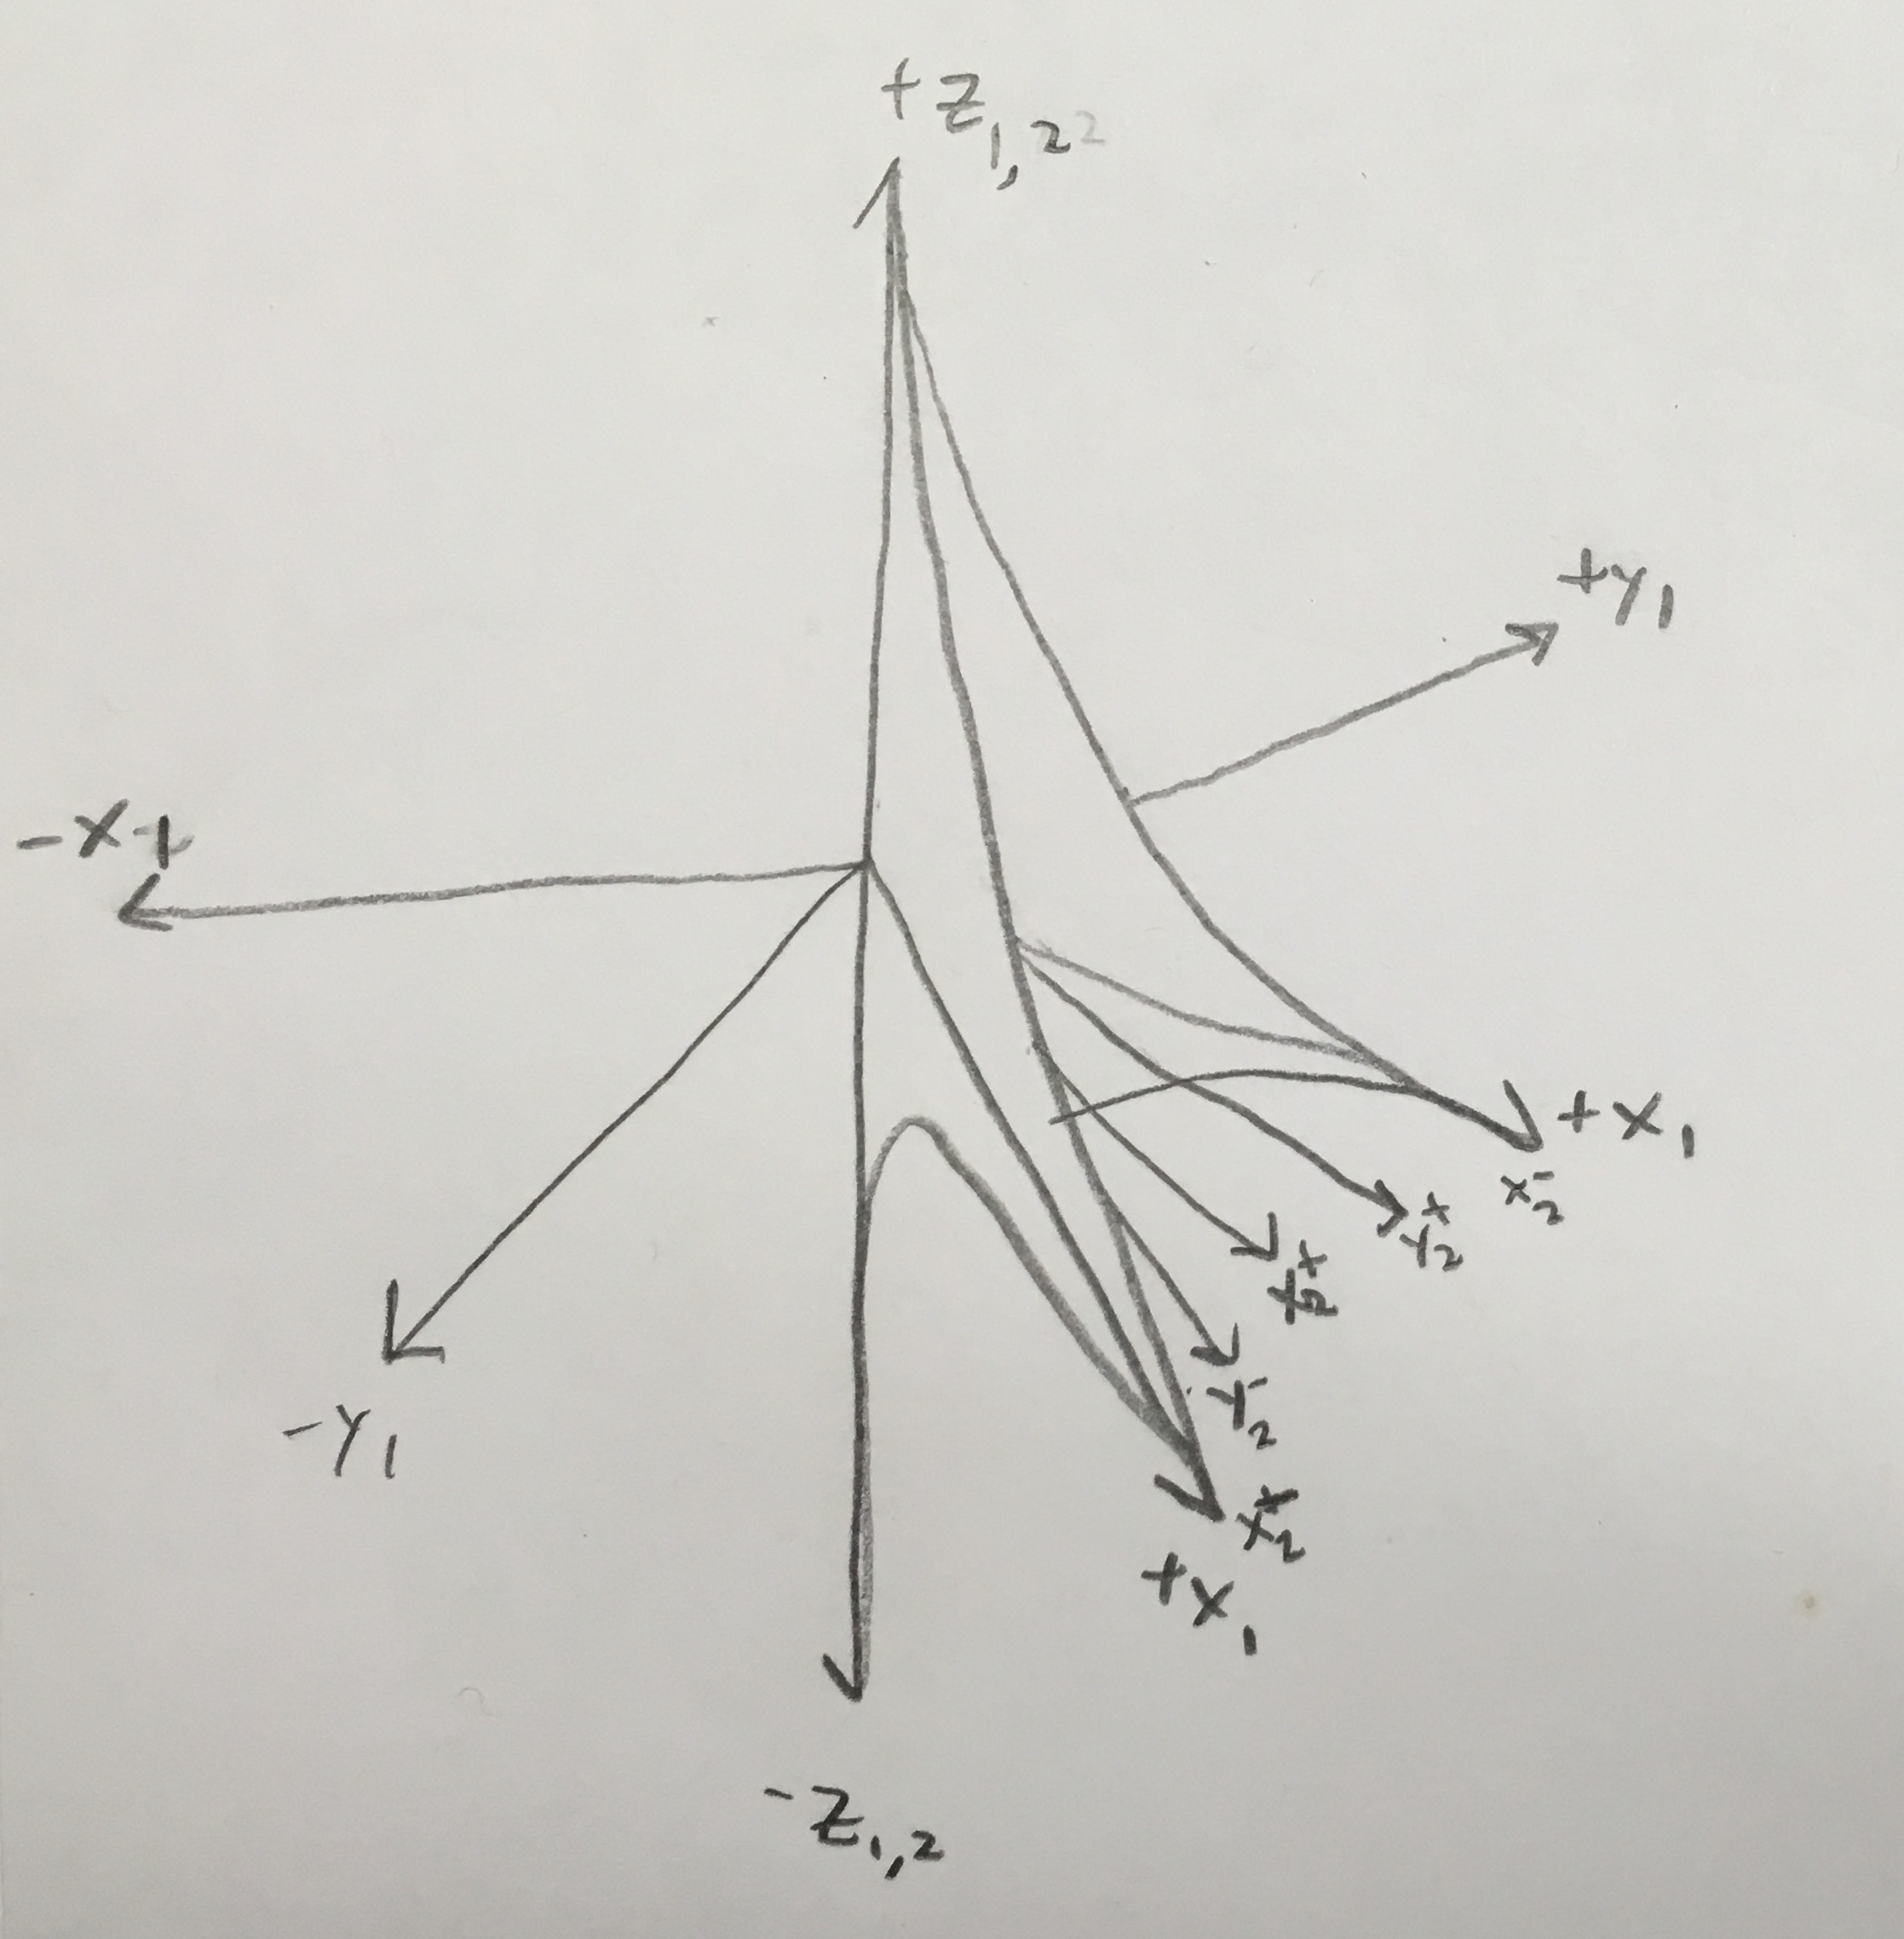
\includegraphics[width=\linewidth]{./figures/fig1.jpg}
	\caption{A 4D line segment split about the z-axis}
	\label{fig:sub1}
   	\end{subfigure}
\end{figure} 

This is where I'd like to introduce the infinite-book concept.  As shown above, we have a four-dimensional line segment. If you notice, there are two 3D spaces here.  
The second space, $<x_2, y_2, z_2>$, is folded between the positive $x$-axis of the first space, and as we continue our motion through the fourth dimension in the direction of the second space, the second space will expand to take up a larger portion of the diagram, and will begin to instead fold the first space behind it until it \textit{"disappears"} from the diagram.

It should be worth noting, that because this space is continuous, if you observe the parts of the diagram that imply some sort of boundary between the two spaces, that there are an uncountable number of spaces in between the two spaces we see here, just as there are an uncountable number of single points between any two points on a line segment.

\begin{figure}[!htbp]
  	\centering
   	\begin{subfigure}[p]{1.0\linewidth}
    	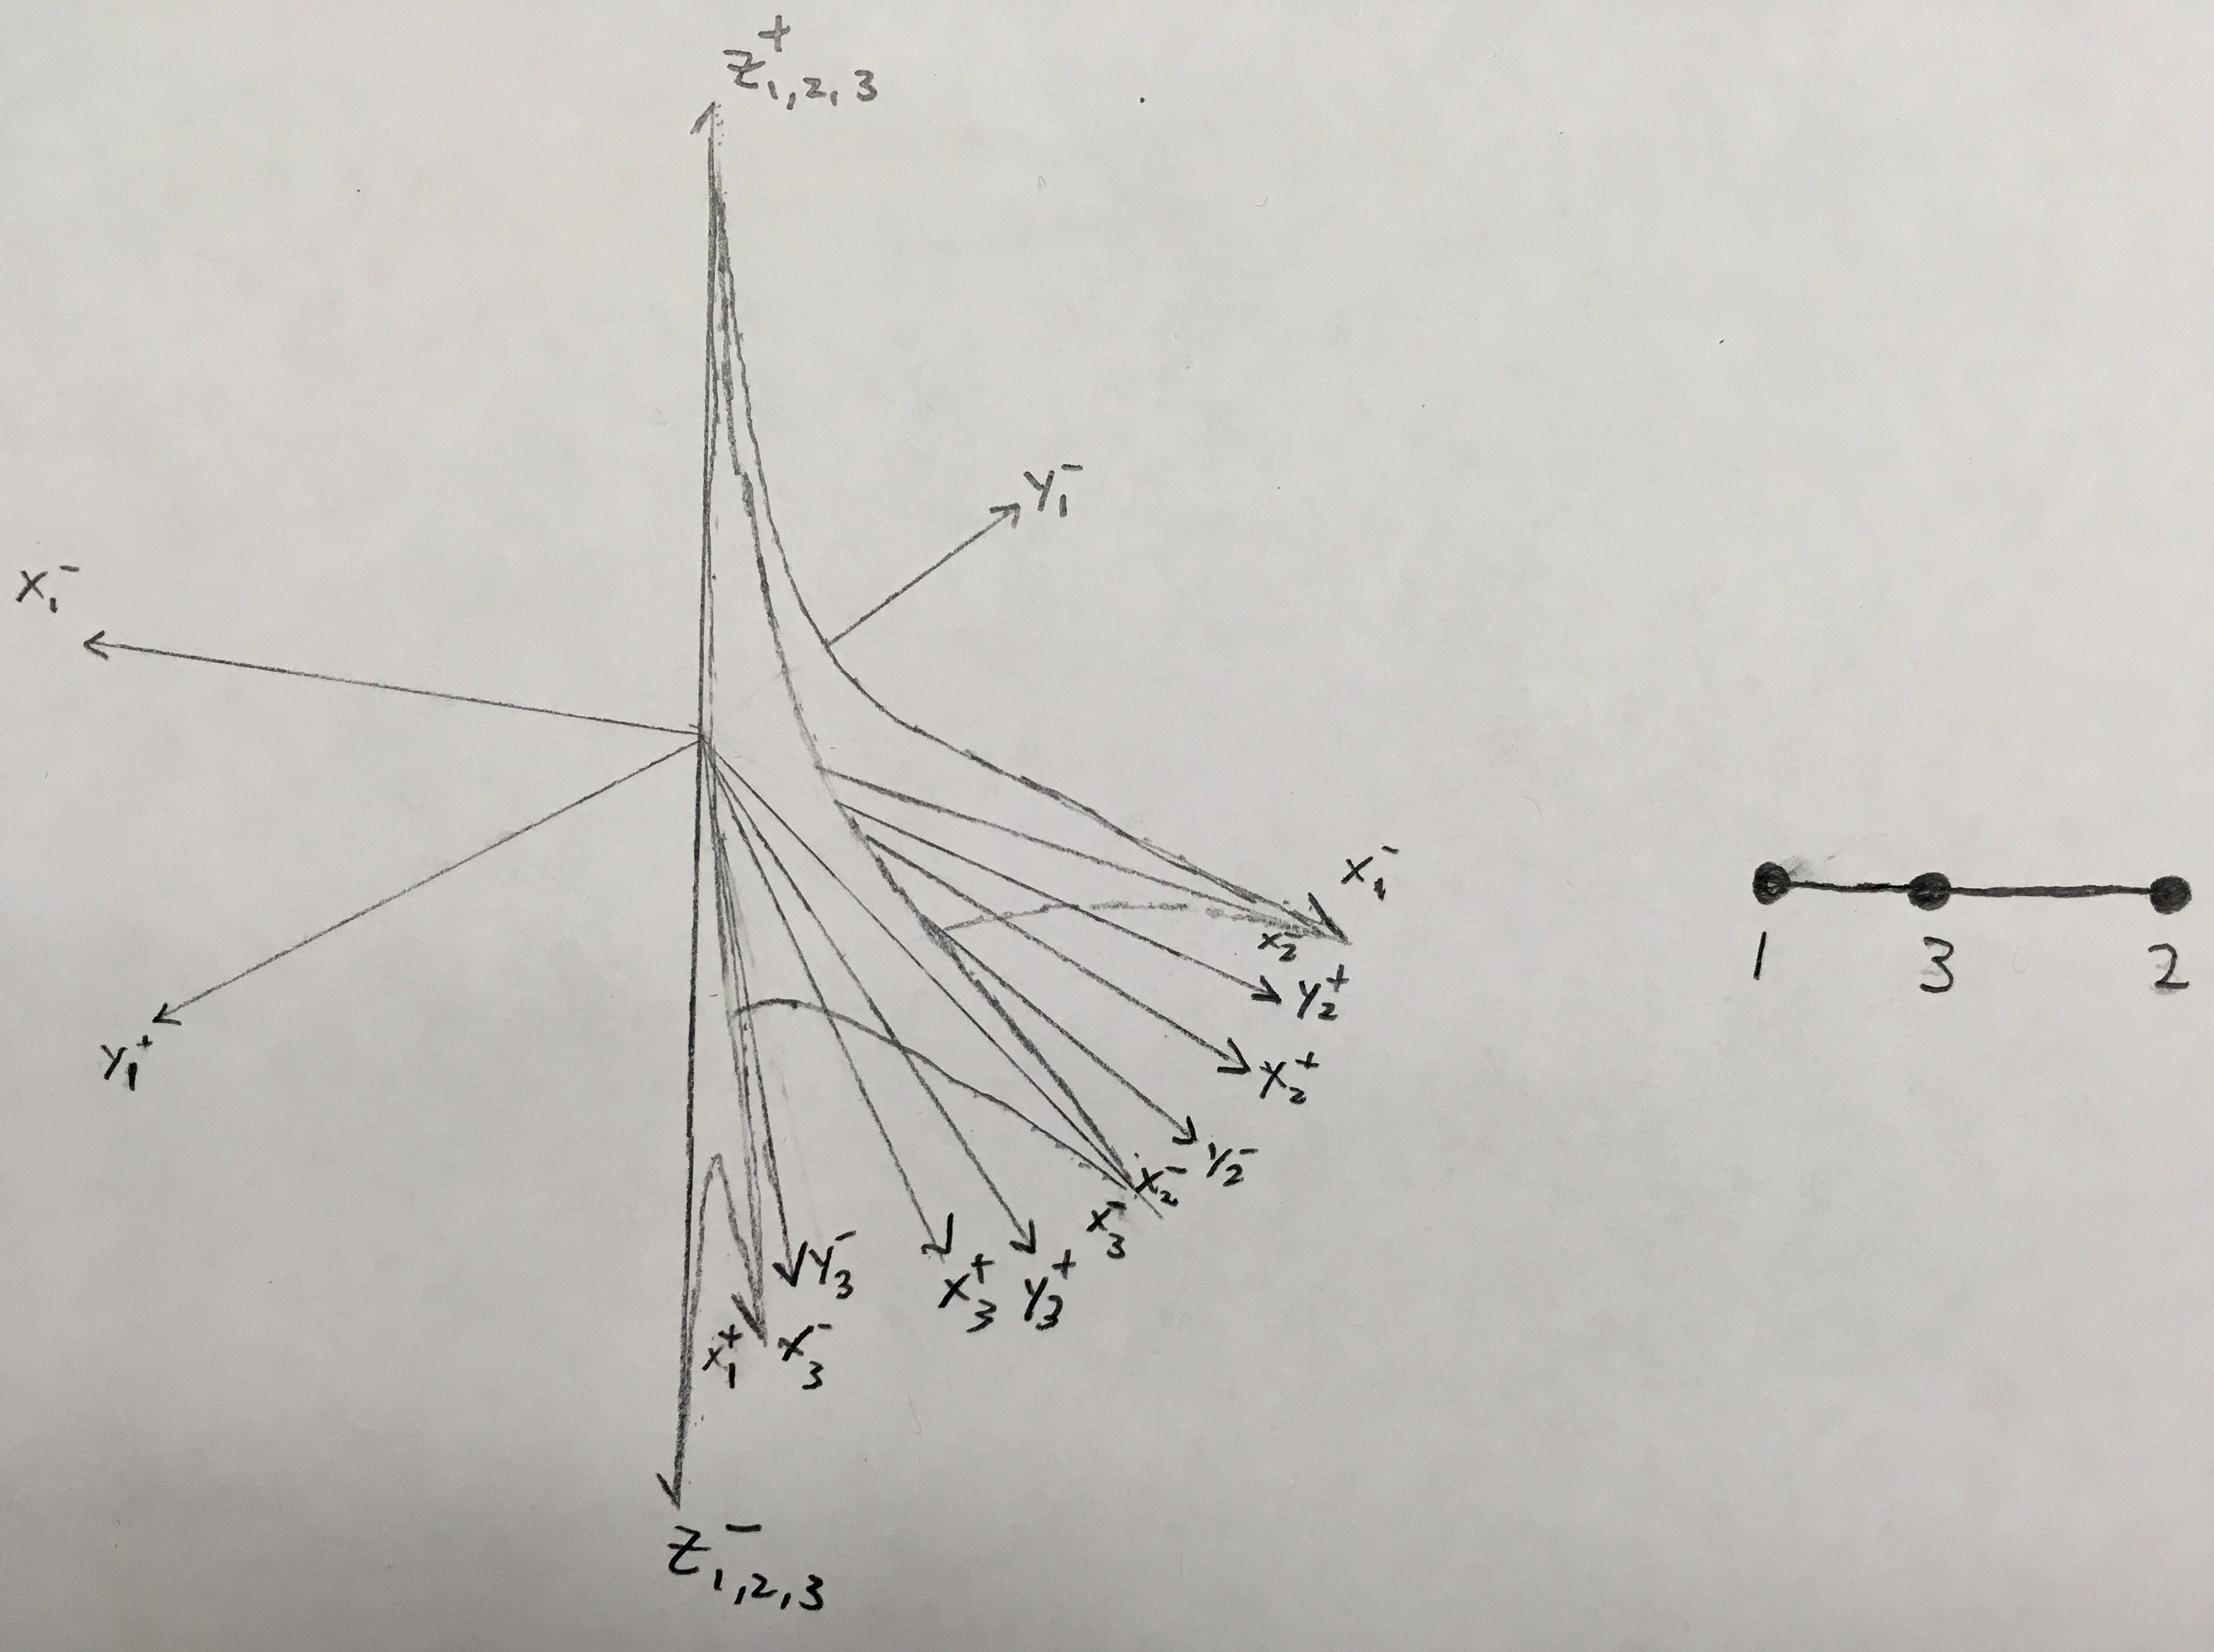
\includegraphics[width=\linewidth]{./figures/fig4.jpg}
	\caption{A 4D line segment with some midpoint and analogous 1D segment}
	\label{fig:sub1}
   	\end{subfigure}
\end{figure} 

As you can see above, we are peeling open one of those boundaries to show yet another space, space $3$, folded between the boundary of the first and second spaces.  I'm not sure yet on how to show this visually, other than assume that $space_1 \leq space_3 \leq space_2$. \\ 

\newpage
There are other questions that can be asked about this diagram, such as: Does the proportion of volume that one space takes up over another in the diagram signify anything? Why does the space split around the $z$-axis like that? I don't have answers to those questions, but I though it would be worthwile to explore some of the different ways in which we could demonstrate traveling between 3D spaces.

\begin{figure}[!htbp]
  	\centering
   	\begin{subfigure}[!p]{0.5\linewidth}
	\centering
    	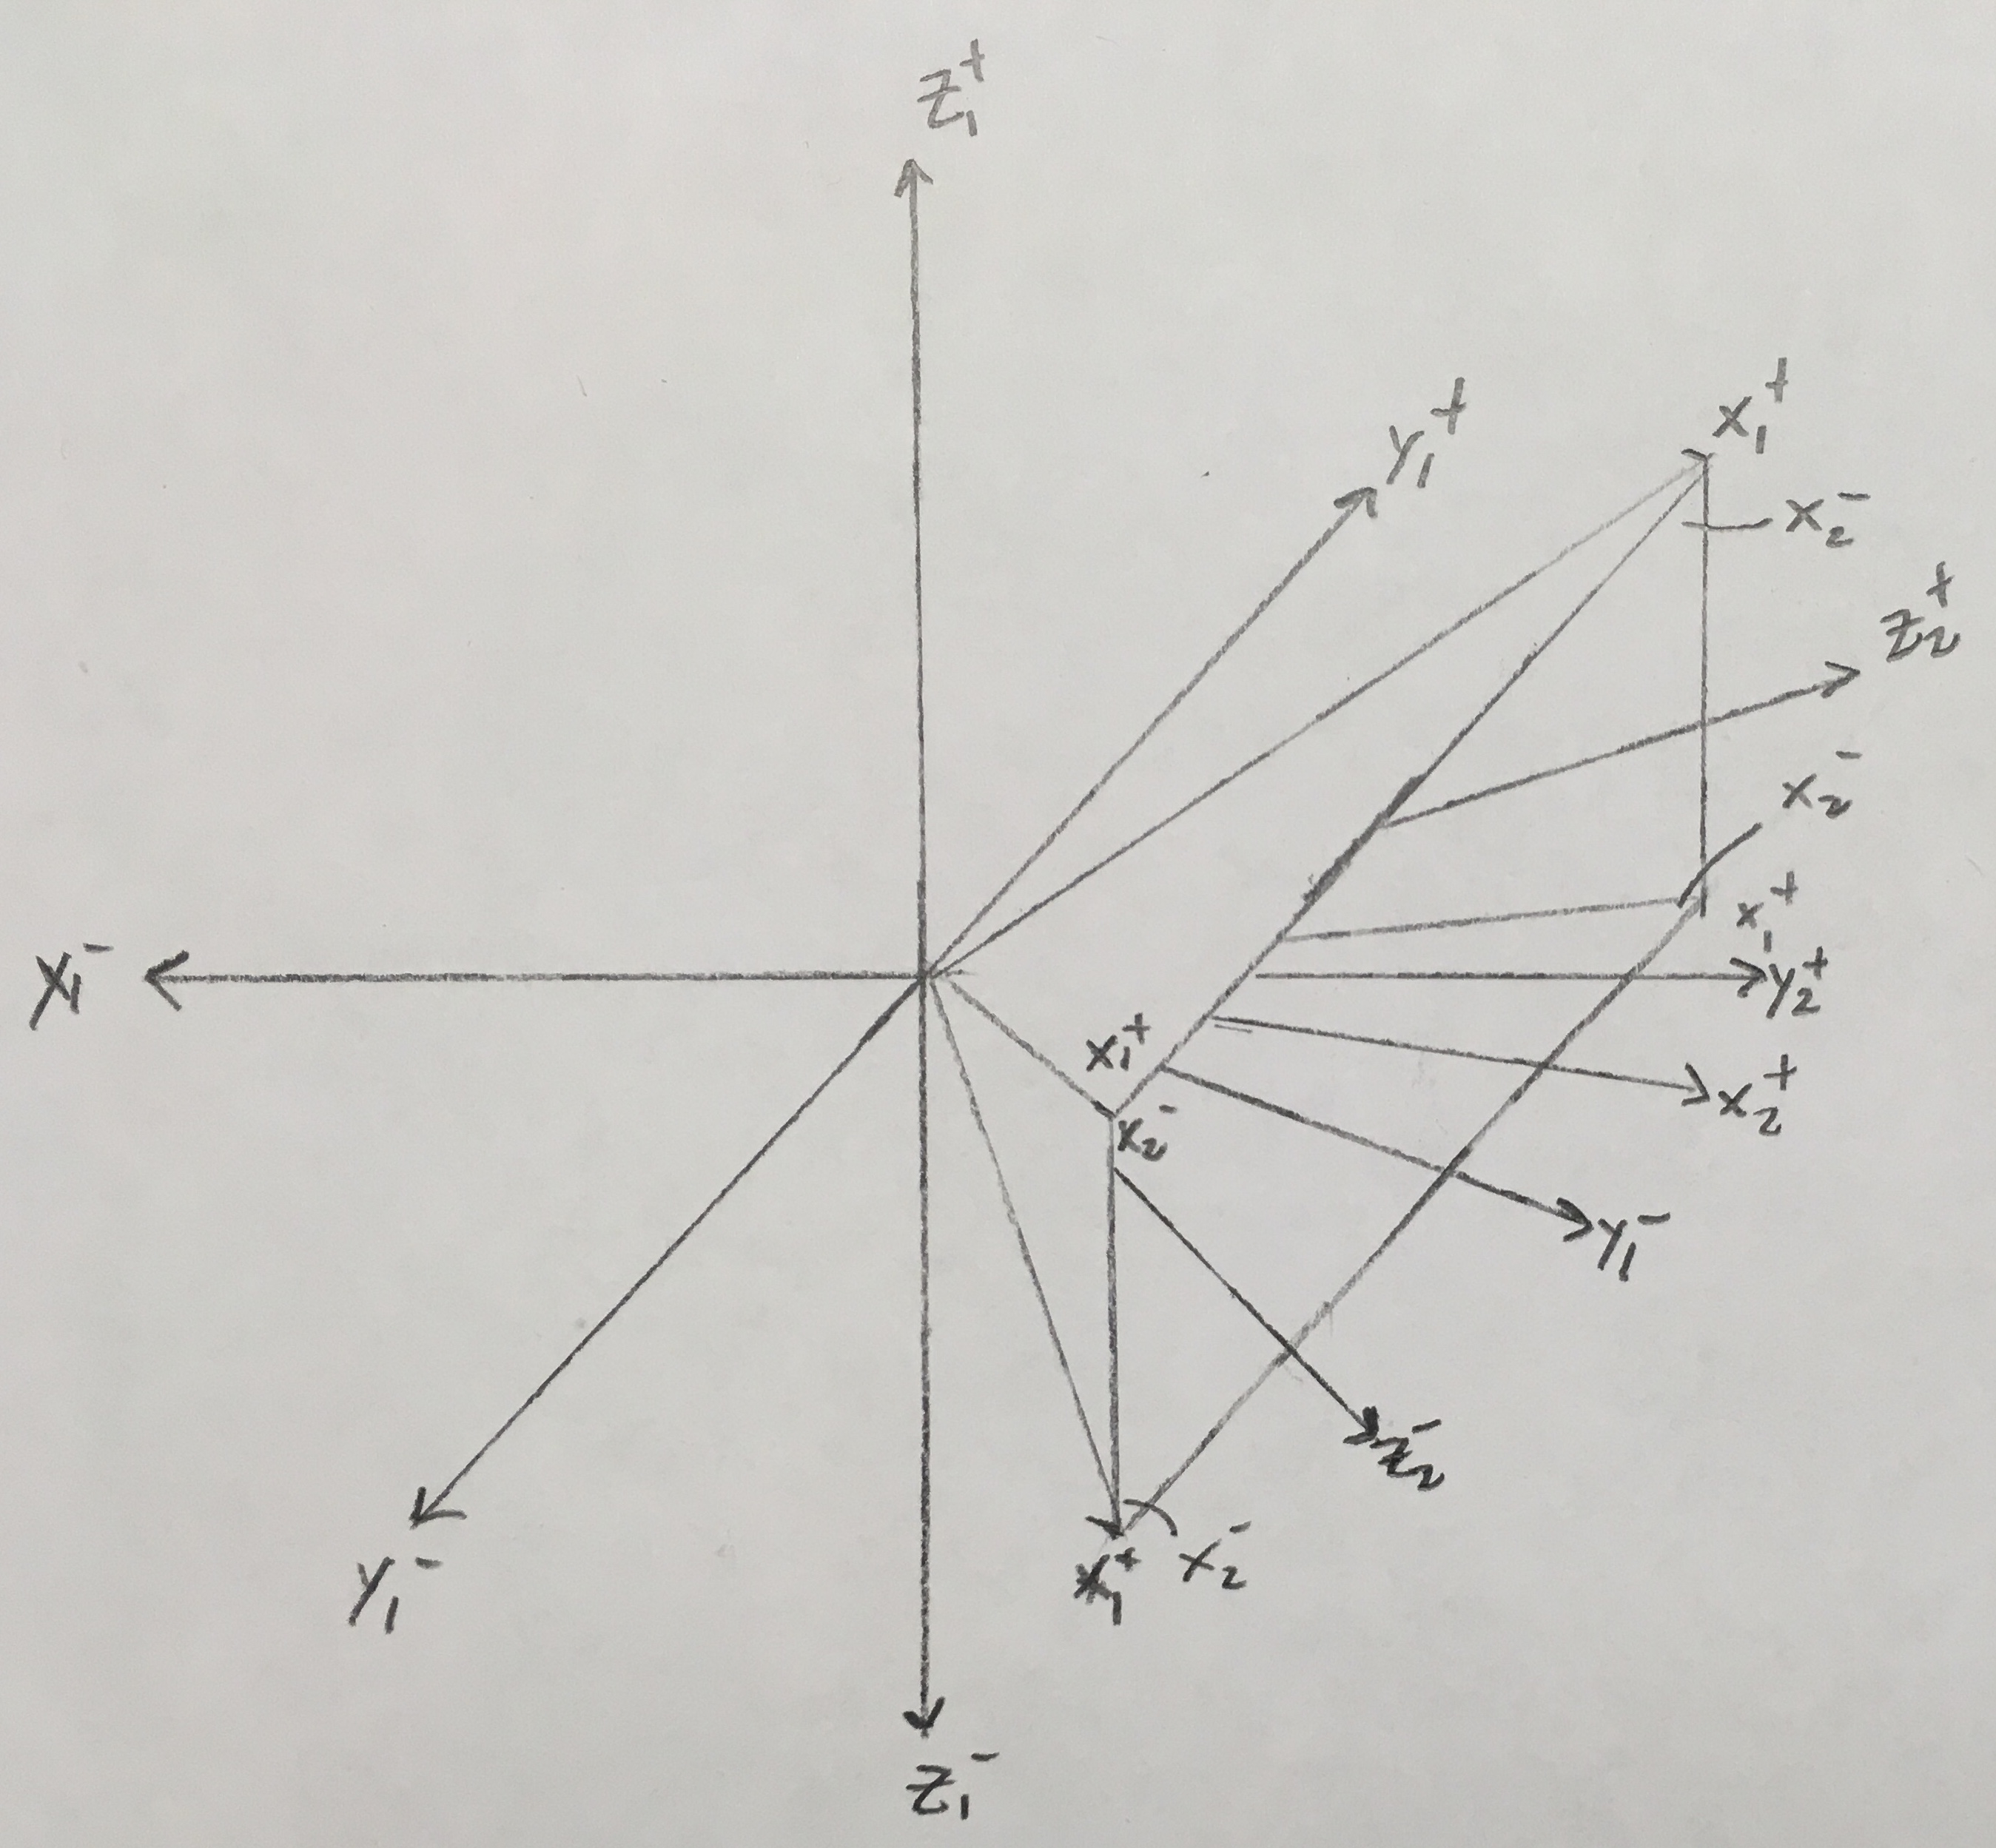
\includegraphics[width=\linewidth]{./figures/fig5.jpg}
	\caption{4D line segment showing a rectangular transition through the $x$-axis}
	\label{fig:sub1}
   	\end{subfigure}
  	\centering
   	\begin{subfigure}[!p]{0.448\linewidth}
	\centering
    	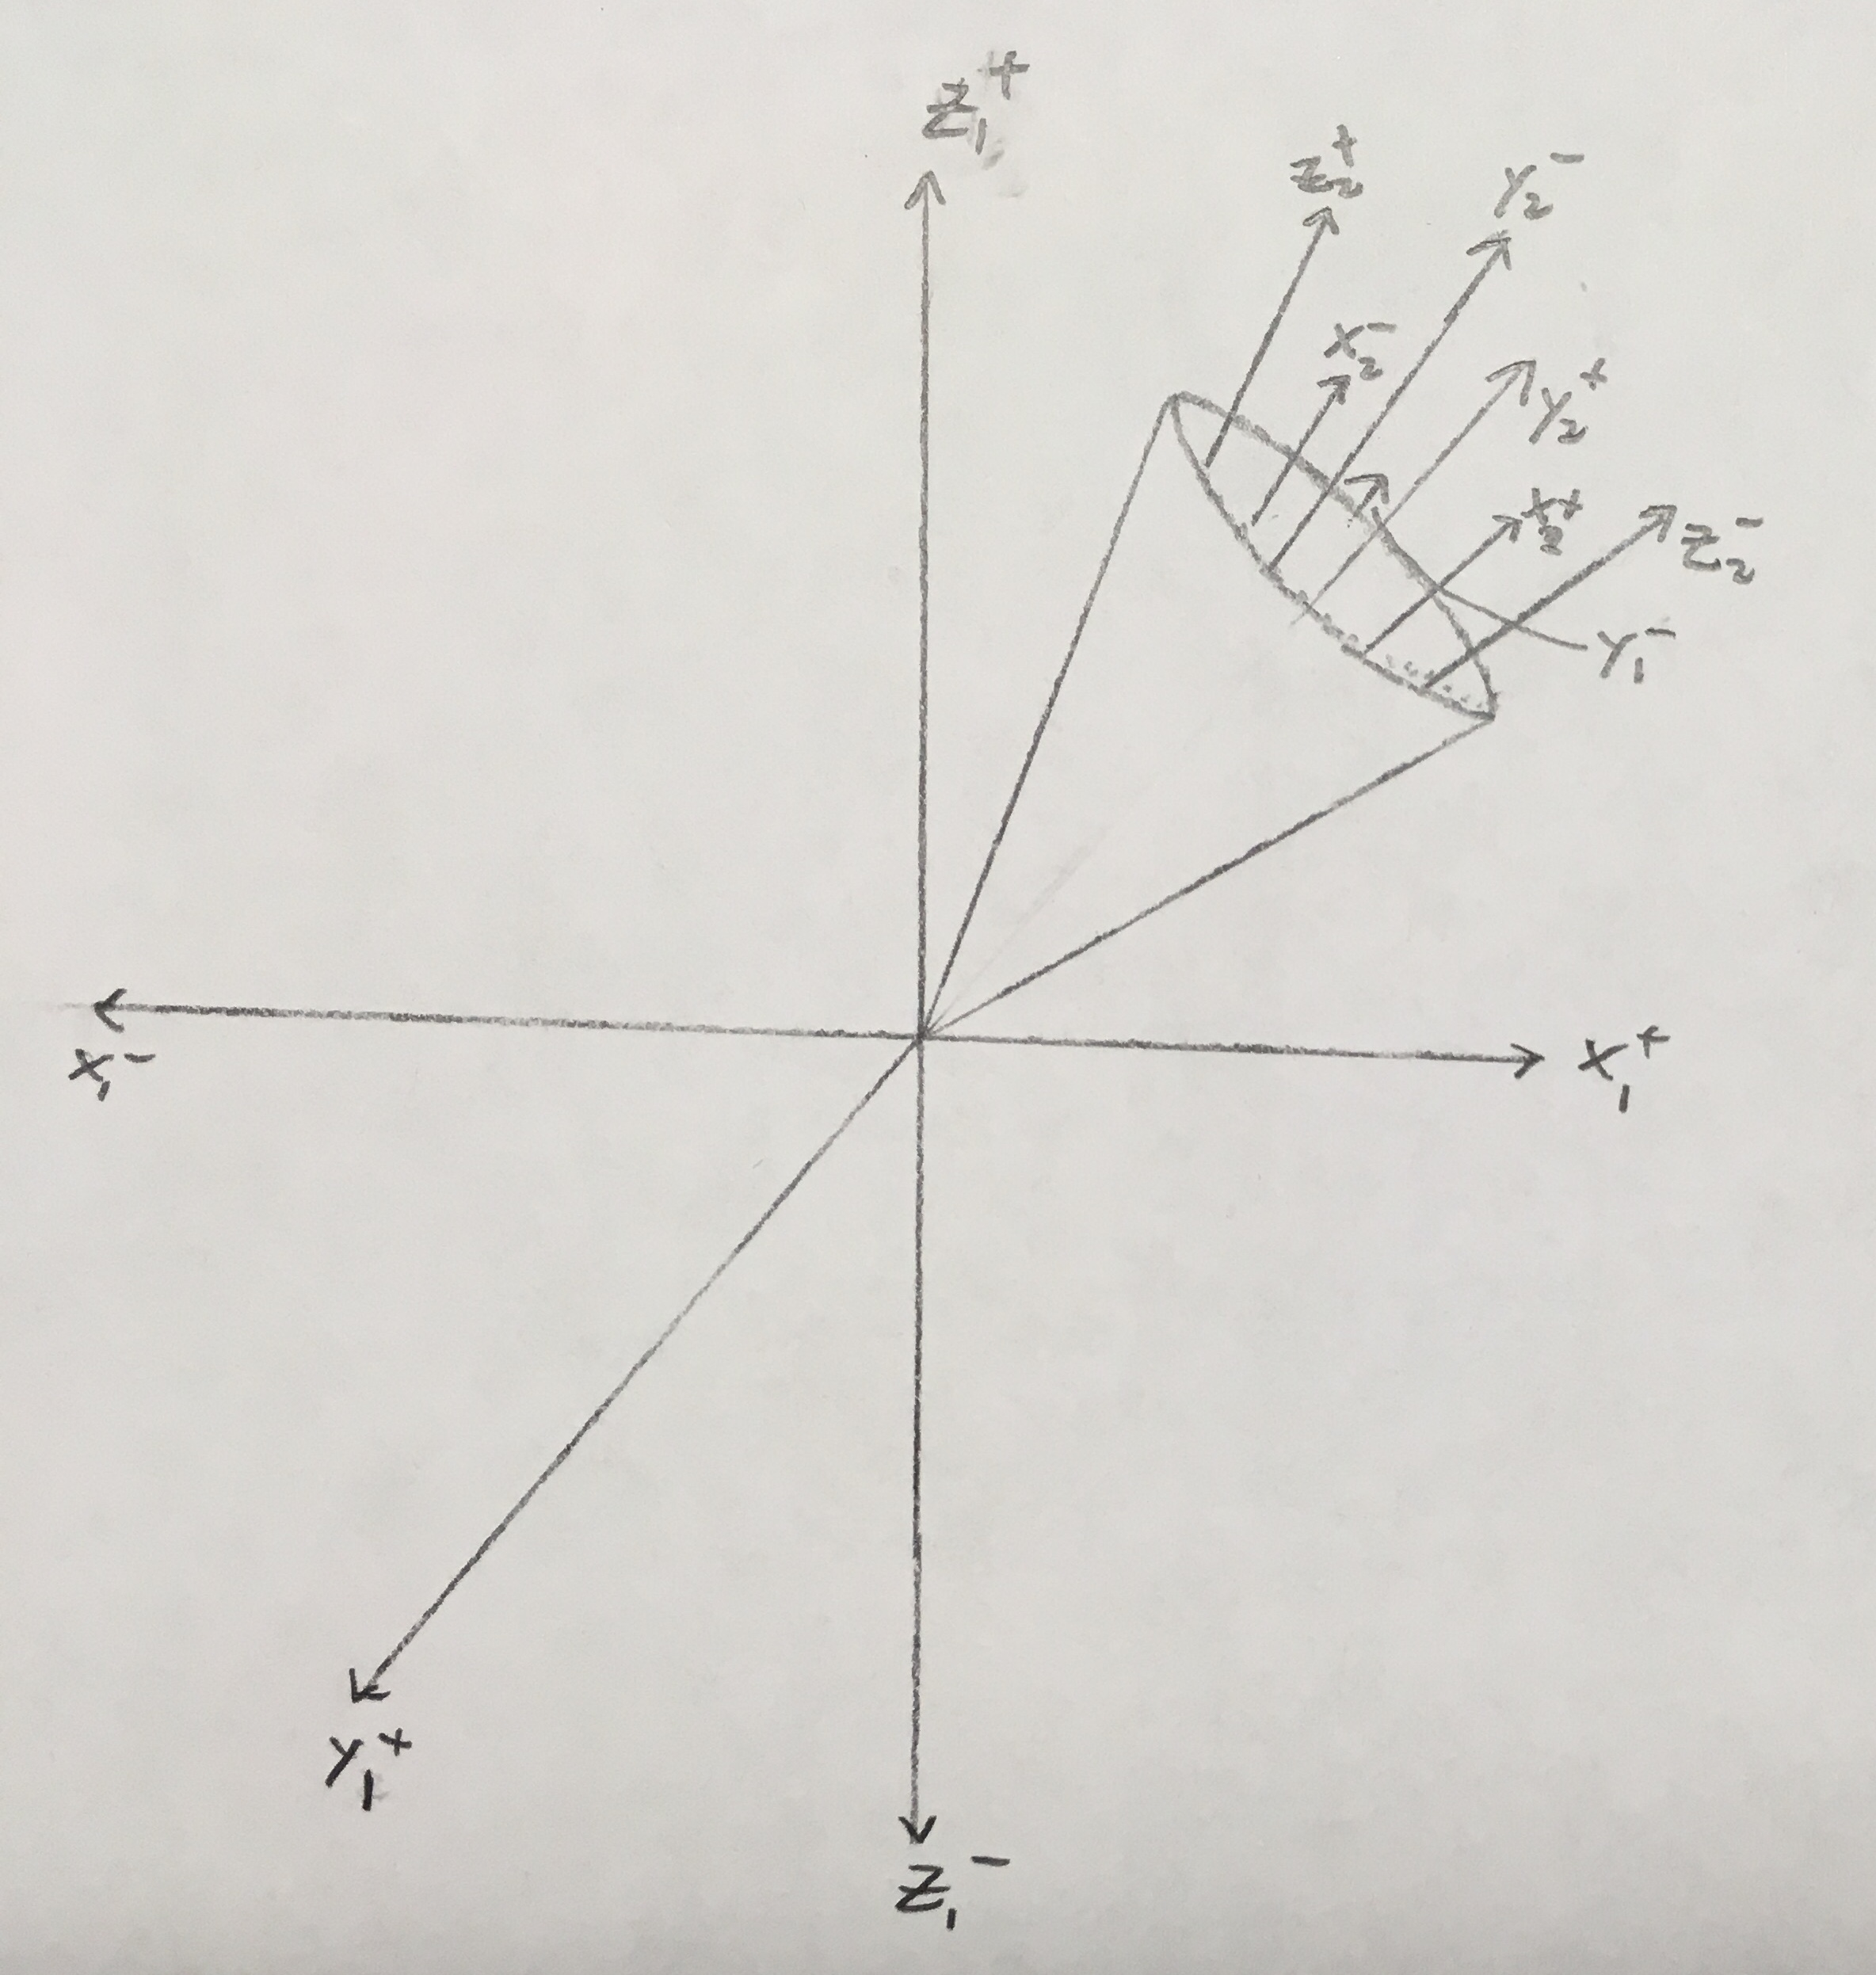
\includegraphics[width=\linewidth]{./figures/fig6.jpg}
	\caption{4D line segment showing a circular transition at an arbitrary angle}
	\label{fig:sub1}
   	\end{subfigure}
\end{figure} 

\begin{figure}[!htbp]
  	\centering
   	\begin{subfigure}[!p]{0.5\linewidth}
	\centering
    	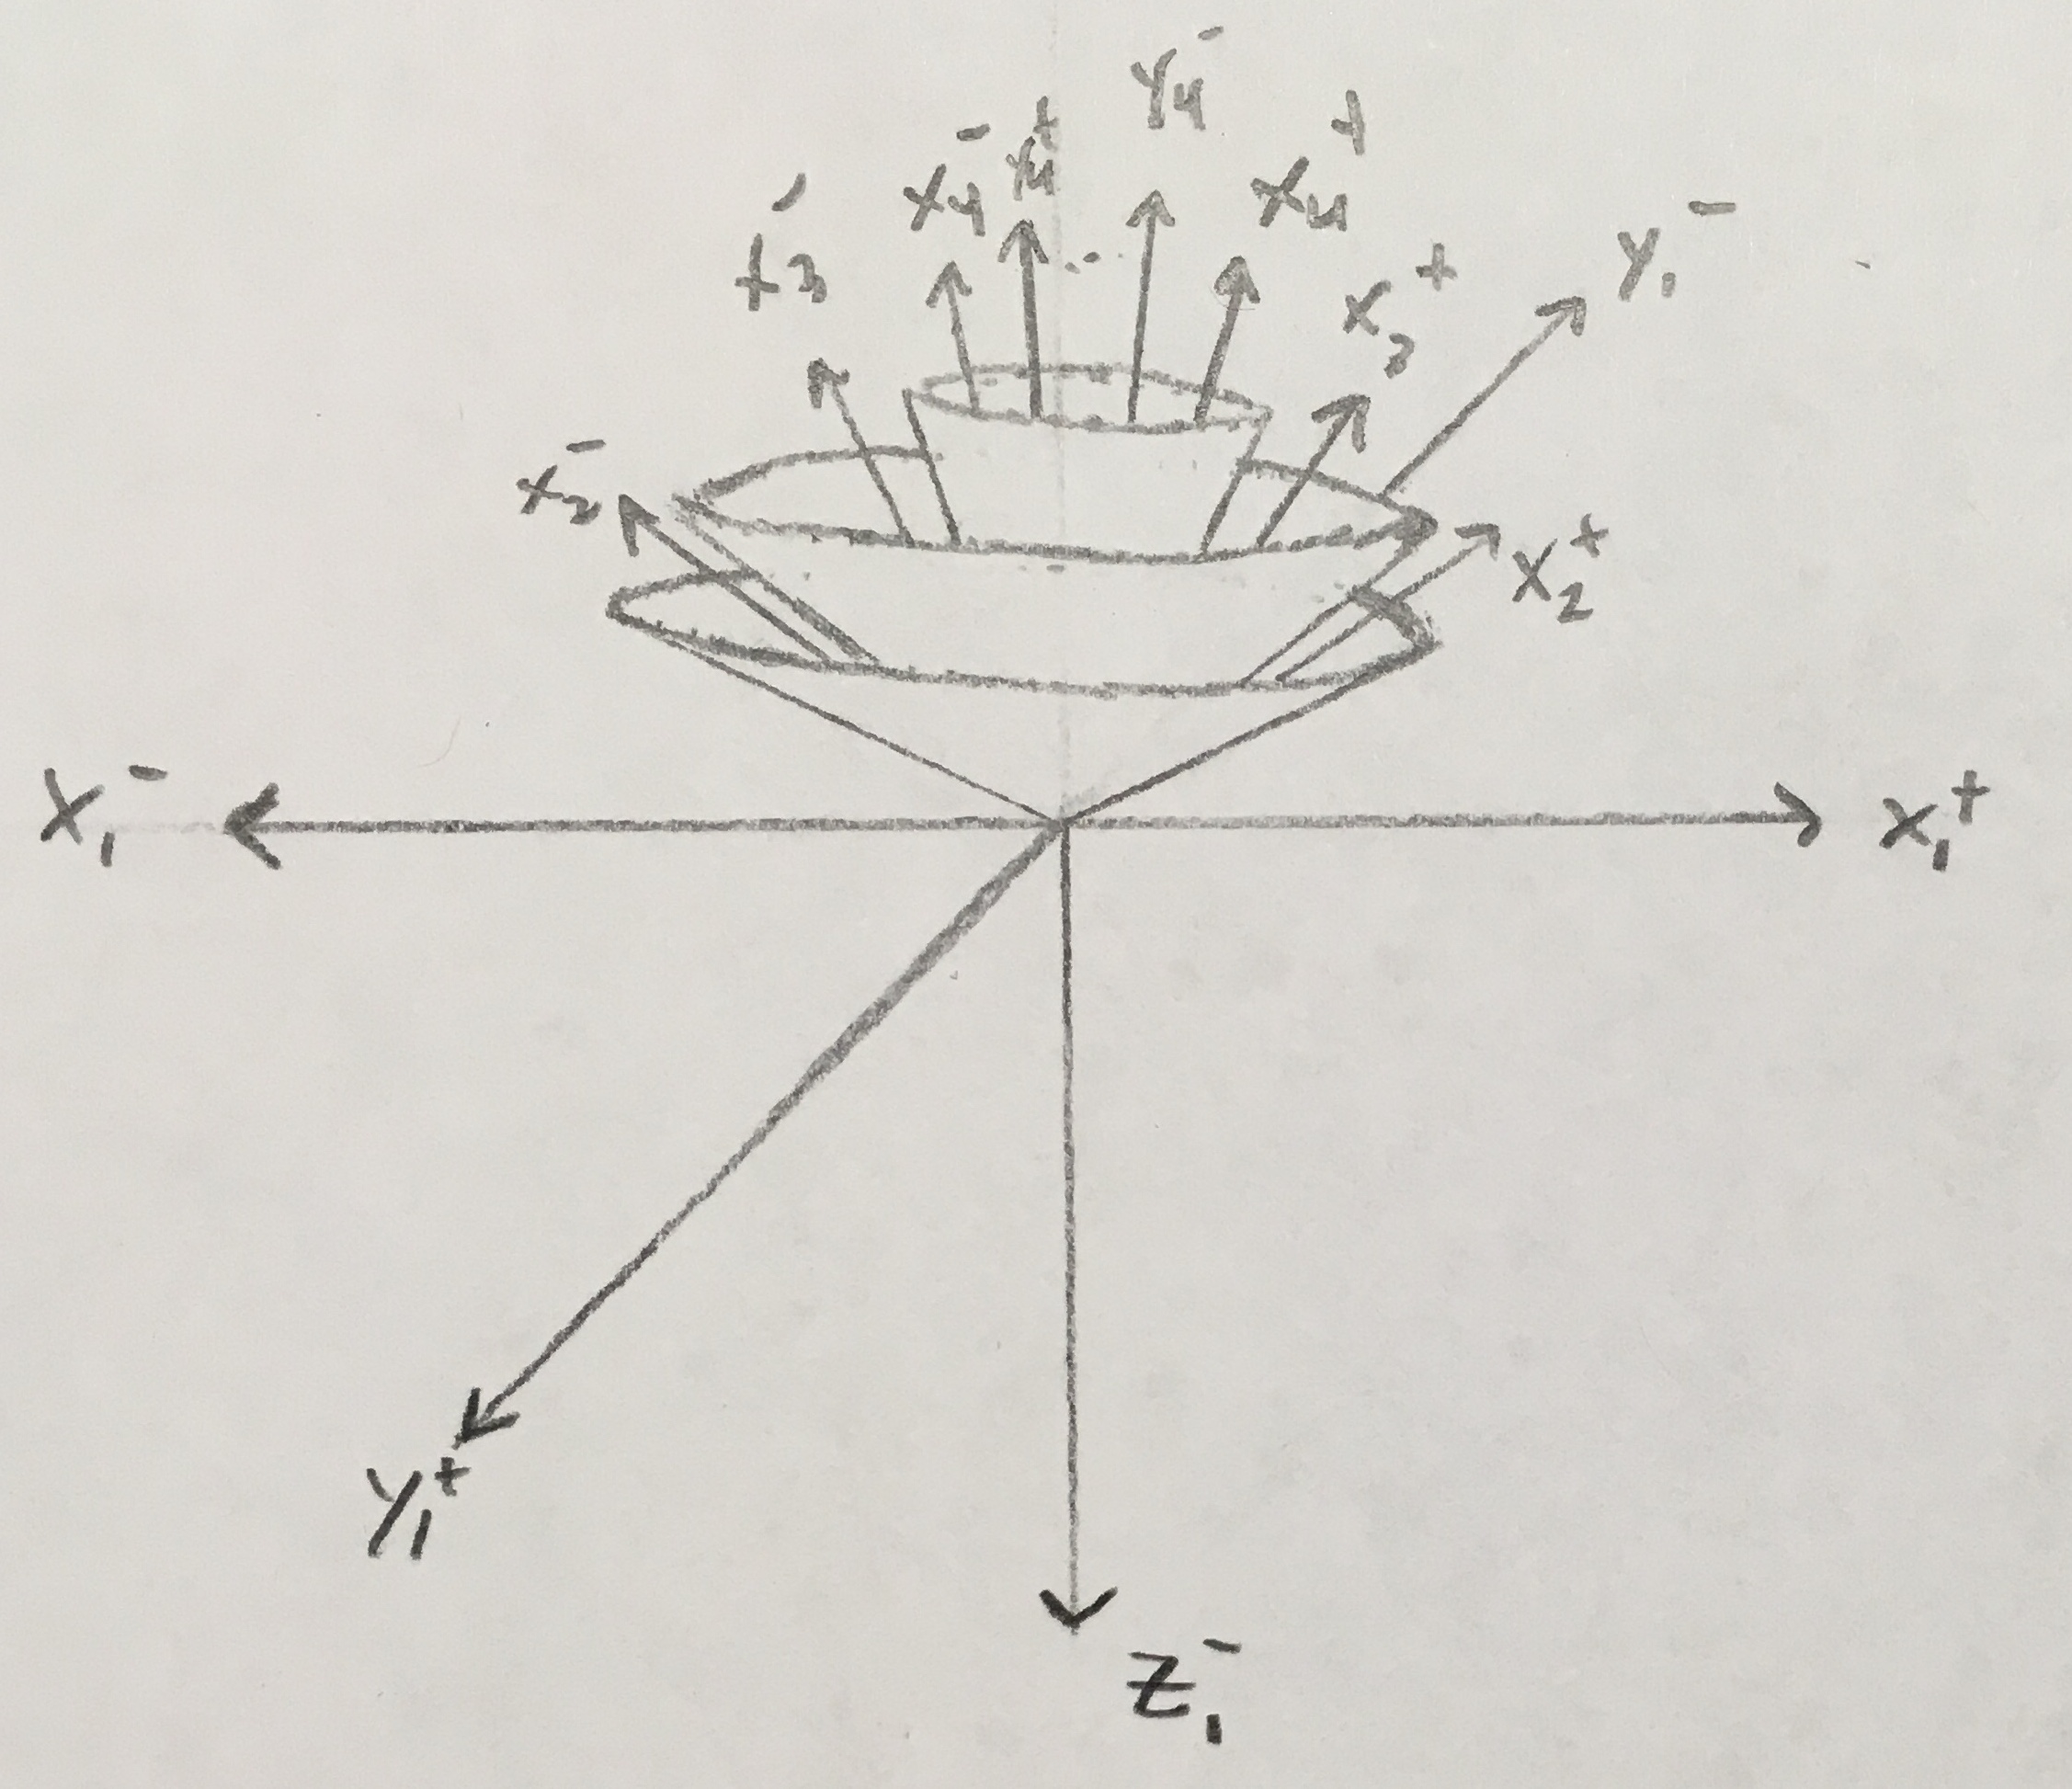
\includegraphics[width=\linewidth]{./figures/fig7.jpg}
	\caption{4D line segment through the $z^{+}$ axis with 2 midpoints}
	\label{fig:sub1}
   	\end{subfigure}
  	\centering
   	\begin{subfigure}[!p]{0.47\linewidth}
	\centering
    	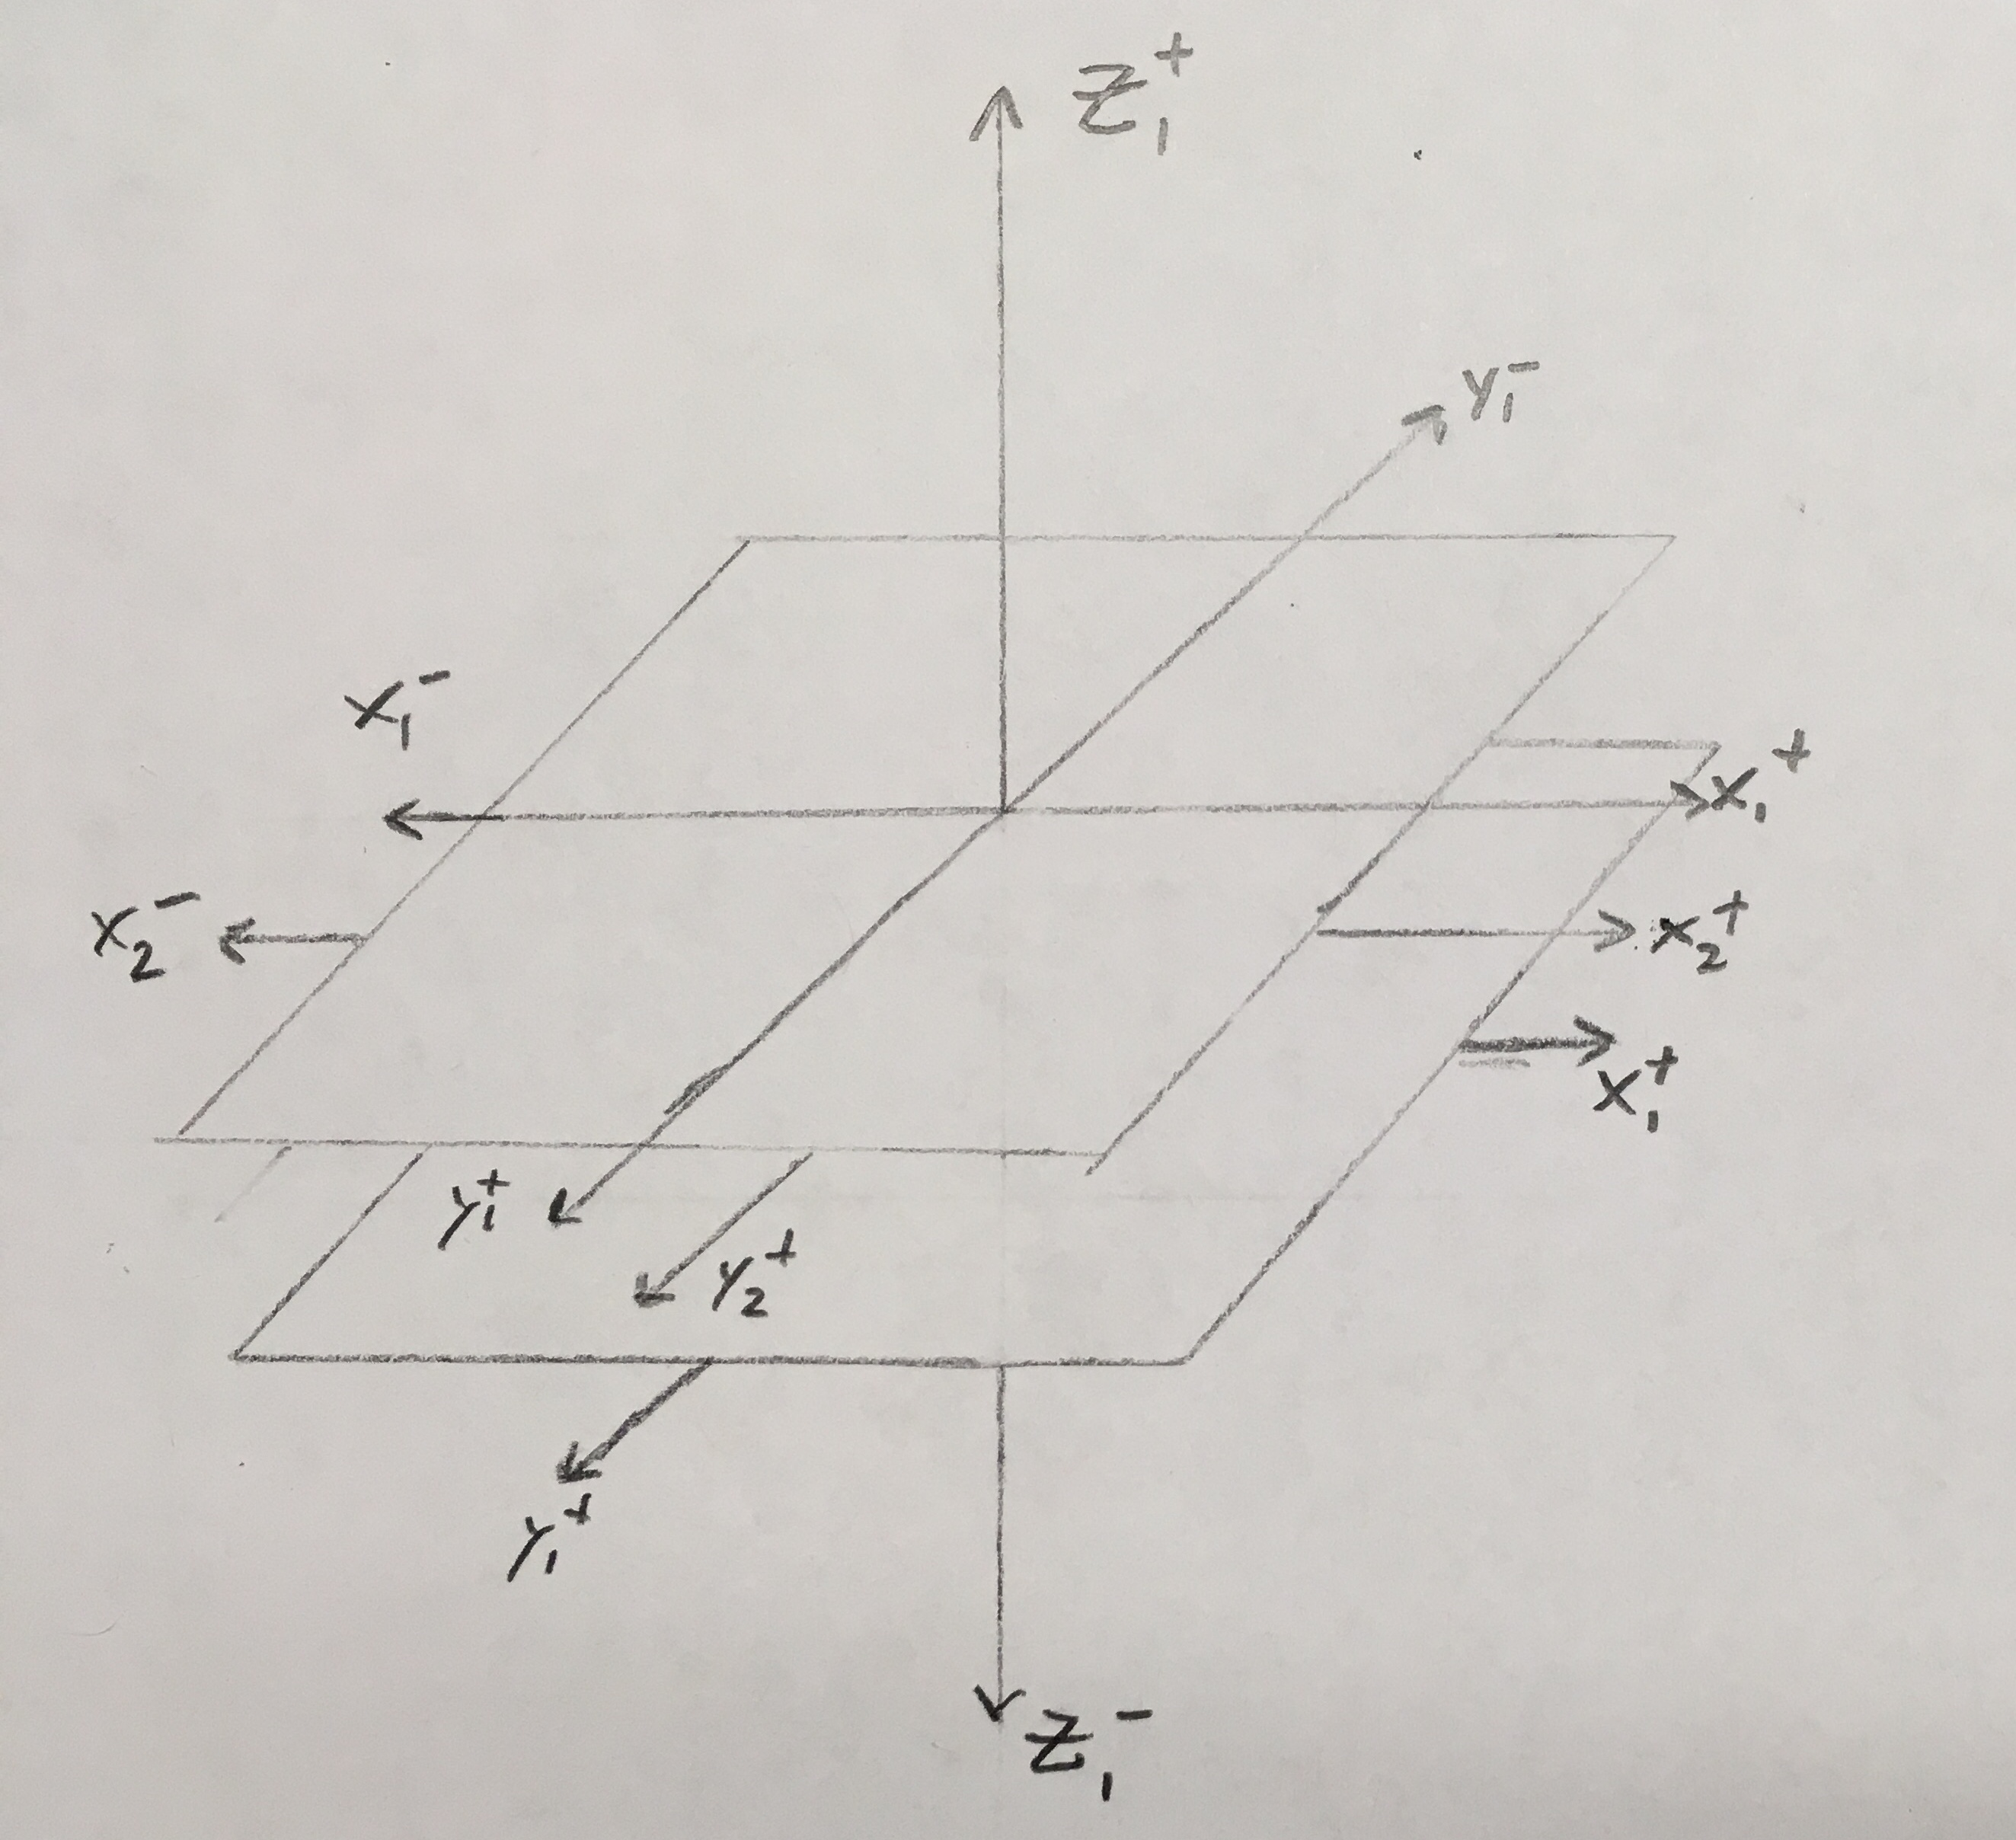
\includegraphics[width=\linewidth]{./figures/fig8.jpg}
	\caption{4D line segment splitting about the $xy$-plane}
	\label{fig:sub1}
   	\end{subfigure}
\end{figure} 


Not all of these could be useful, provable, or feasible, but I think it's useful to at least explore these different implementations of the model to aid in understanding and developing it.


\end{document}










































